\documentclass{beamer}
\usetheme{Boadilla}
\usepackage{xcolor, soul}
\sethlcolor{red}
\usepackage[absolute,overlay]{textpos}
\usepackage[ruled,vlined]{algorithm2e}
\usepackage{dsfont}
\usepackage{array}
\usepackage{tikz}
\usetikzlibrary{shapes, arrows.meta, positioning}
\usepackage[style=alphabetic]{biblatex}  
\addbibresource{lib.bib}
\usepackage{caption}
\usepackage{xcolor}



\author[Jonas Müller]{Jonas Carsten Reinhard Müller}


\setbeamertemplate{enumerate item}{\arabic{enumi}.}  % Use regular numbers and a period
%%%%%%%%%%%%%%%%%% Begin of the Presentation %%%%%%%%%%%%%%%%%

\begin{document}
\title[Boosting]{A Theory of Multiclass Boosting}
\subtitle[short subtitle]{Paper by Schapire and Mukherjee \cite{mukherjee2011theory}}
\institute{}
\date{}

\begin{frame}
    \titlepage
\end{frame}

%%%%%%%%%%%%%%%%%% Outline %%%%%%%%%%%%%%%%%%%%%

\section{Foundation}
\subsection{What is Boosting?}
\subsection{AdaBoost}
\section{Regarding the Theory}
\subsection{Why the need for Theory?}
\subsection{The Boosting Game}
\subsection{What is a 'good' weak-learner?}
\subsection{New Algorithm}
\section{Discussion}
\subsection{Outlook}


% table of contents 
\begin{frame}
    \frametitle{Outline}
    \tableofcontents
\end{frame}


%%%%%%%%%%%%%%%%%% Beginning of slides %%%%%%%%%%%%%%%%%


\begin{frame}{What is Boosting?}
    \centering
    \begin{itemize}
        \item Utilizing Wisdom of the Crowd
        \item Many so called weak-learners are combined into one strong classifier
    \end{itemize}
    \bigbreak
    \begin{center}
        \begin{columns}
            \begin{column}{0.6\hsize}
                \centering
                \tikzstyle{start} = [ellipse, draw, fill=blue!20,
                text width=3.5em, text centered, node distance=1.5cm, minimum height=1.5em]
                \tikzstyle{result} = [rectangle, draw, fill=green!20,
                text width=6em, text centered, rounded corners, minimum height=3em]
                \tikzstyle{result2} = [rectangle, draw, fill=red!20,
                text width=6em, text centered, rounded corners, minimum height=3em]
                \tikzstyle{line} = [draw, -]

                \begin{tikzpicture}[node distance = 2.5cm, auto]
                    % Place nodes
                    \node [start] (start) {Raining?};
                    \node [result, below left of=start] (Accept) {Wear a Jacket};
                    \node [result2, below right of=start] (Reject) {Don't Wear a Jacket};

                    % Draw edges
                    \path [line] (start) -- node {Yes}(Accept);
                    \path [line] (start) -- node {No}(Reject);
                \end{tikzpicture}
                \captionof{figure}{\small A simple decision Stump}
            \end{column}
            \begin{column}{0.4\hsize}
                \begin{figure}
                    \centering
                    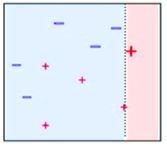
\includegraphics[width=0.8\linewidth]{images/weaklearner.JPG}
                    \caption{\small Weak-Learner in \cite{MultiAna}}
                    \label{fig:example}
                \end{figure}
            \end{column}
        \end{columns}
    \end{center}
\end{frame}

\begin{frame}[fragile]
    \frametitle{AdaBoost}
    \small
    \begin{algorithm}[H]
        \captionsetup{labelformat=empty}
        \KwData{Training set $S = \{(x_1, y_1), (x_2, y_2), \ldots, (x_m, y_m)\}$, where $x_i$ is a feature vector and $y_i \in \{-1,1\}$ is a label.}
        \KwResult{Classifier $H$.}
        Initialize distribution $D_1(i) = \frac{1}{m}$ for $i = 1, 2, \ldots, m$ \\
        \For{$t=1$ \KwTo $T$}{
            Train weak learner $h_t(x)$ using distribution $D_t$ \\
            Compute error: $\varepsilon_t = \sum_{i=1}^m D_t(i) \cdot \mathds{1}[h_t(x_i) \neq y_i]$ \\
            Compute classifier weight: $\alpha_t = \frac{1}{2} \ln\left(\frac{1 - \varepsilon_t}{\varepsilon_t}\right)$ \\
            Update distribution: $D_{t+1}(i) = D_t(i) \cdot \exp(-\alpha_t \cdot y_i \cdot h_t(x_i))$ for $i \in [m]$ \\
            Normalize $D_{t+1}$ \\
        }
        Final strong classifier: $H(x) = \text{sign}(f(x))$ with $f(x) = \left(\sum_{t=1}^T \alpha_t \cdot h_t(x)\right)$
        \caption{AdaBoost in \cite{schapire2013explaining}}
    \end{algorithm}
    \begin{itemize}
        \item There exist different Multiclass extensions of this.
        \item We minimize the convex loss function $L(x,y) = e^{-yf(x)}$.
    \end{itemize}
\end{frame}


\begin{frame}{Why the need for Theory?}
    \centering
    \begin{itemize}
        \item Binary setting has a theoretical Foundation. \\
              $\rightarrow$ Such an Understanding is lacking in the Multiclass setting. \\
        \item Goal: Create a Framework that captures known Algorithms and utilize that to derive new ones.
    \end{itemize}
    \begin{figure}
        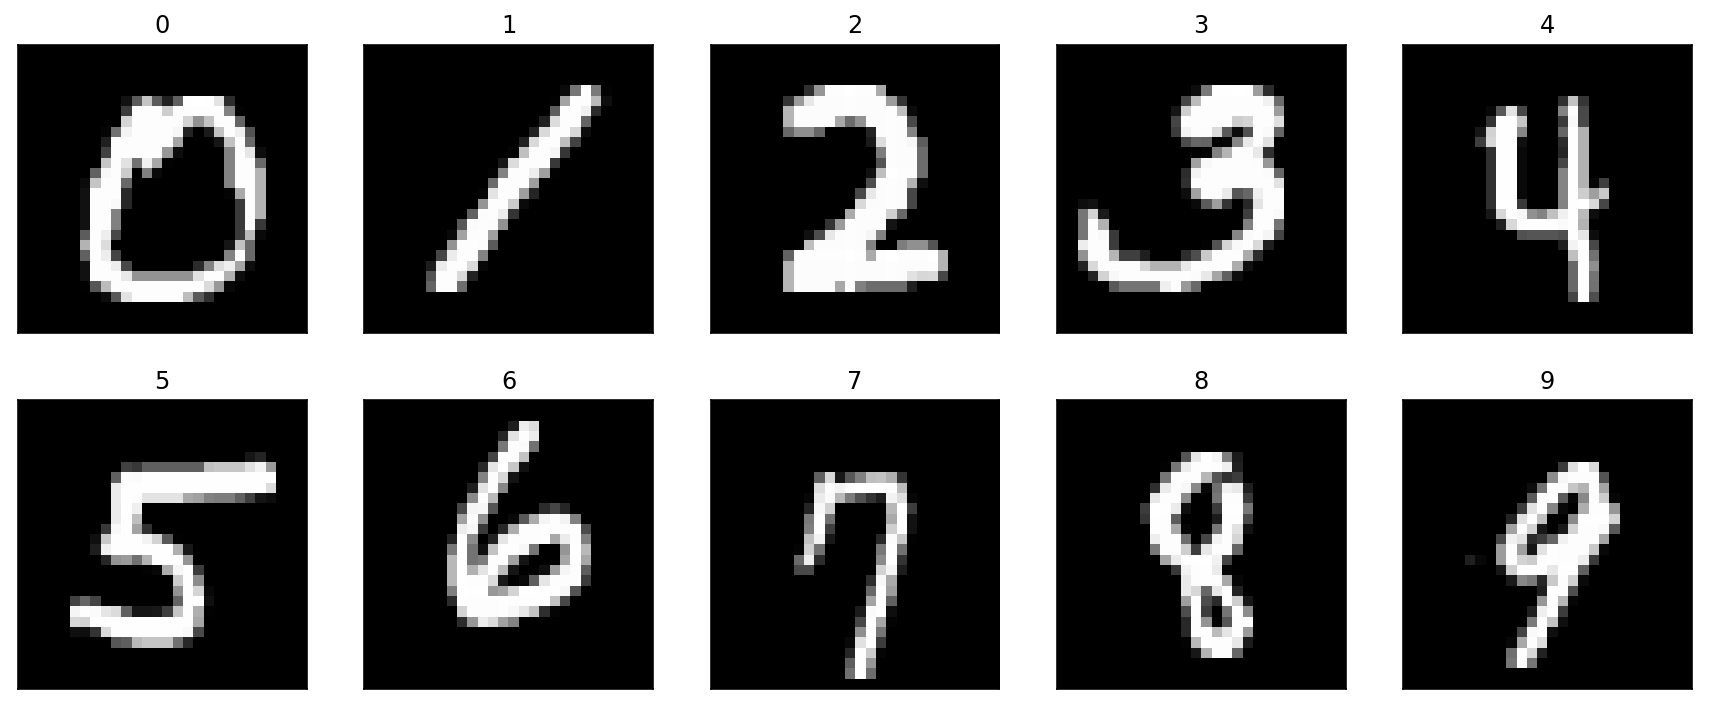
\includegraphics[width=0.8\linewidth]{images/mnist-486535952.png}
        \caption{\small MNIST dataset example}
        \label{fig:MNIST}
    \end{figure}
\end{frame}

\begin{frame}{The Boosting Game}
    Game is played for $T$ rounds, round $t \in [T]$ plays out as follows:
    \bigbreak
    \begin{enumerate}
        \item Booster creates some cost matrix $C_t \in \mathbb{R}^{m,k}$
        \item Weak-Learner returns weak classifier $h_t: X \rightarrow \{1, \dots ,k\}$ with $h_t \in \mathcal{H}$ such that the cost is somewhat 'small'
        \item Based on the cost, Booster computes some weight $\alpha_t$ for this round
    \end{enumerate}
    \bigbreak

    After the end, the final classifier is:
    \begin{center}
        $H(x) = \underset{l \in \{1,...,k\}}{\text{argmax}} \sum_{1 = i}^{T} \alpha_i \cdot \mathds{1} [h_i(x) = l]$
    \end{center}
\end{frame}


\begin{frame}{What are 'good' weak-learning conditions? (1)}
    We call  $(\mathcal{C}, B)$ a \textbf{\textcolor{blue}{Weak-Learning-condition}}. \\
    $\mathcal{C} \subseteq \mathbb{R}^{m,k}$ defines what kind of costs are allowed. \\
    $B \in \mathbb{R}^{m,k}$ is a Baseline that defines how much better than random the weak-learners need to be.

    \bigbreak

    A space $\mathcal{H}$ satisfies $(\mathcal{C},B)$ if for all $C \in \mathcal{C}$ there is some $h \in \mathcal{H}$ such that:
    \begin{center}
        $\sum_{i = 1}^{m} C(i, h(i)) \leq \sum_{i = 1}^{m} \langle C(i), B(i)\rangle$ \\
    \end{center}
    \bigbreak
    \textbf{\textcolor{blue}{In short:}} For every Cost Matrix, there needs to be a classifier that beats the Baseline.
\end{frame}

\begin{frame}{What are 'good' weak-learning conditions? (2)}
    \textbf{\textcolor{blue}{Boostable Spaces}} $\mathcal{H}$ \\
    We say $\mathcal{H}$ is Boostable if there is some distribution $\lambda$ over $\mathcal{H}$ such that: \\
    \begin{center}
        $\sum_{h \in \mathcal{H}} \lambda(h) \cdot \mathds{1}[h(x_i) = l] = y_i$ for all $i \in [m]$
    \end{center}
    \bigbreak
    \textbf{\textcolor{red}{Goal:}} Find $(\mathcal{C},B)$ such that $\mathcal{H}$ satisfies $(\mathcal{C}, B)$ if and only if $\mathcal{H}$ is Boostable. \\
    \bigbreak
    \textbf{\textcolor{blue}{Formalizing the Intuition:}} Edge-over-random \\
    Let $\mathcal{C}^{eor} \subseteq \mathbb{R}^{m,k}$ be the set of matrices where the rows come from $\{c \in \mathbb{R}^k \mid \forall l: c(1) \leq c(l)\}$ (we assume 1 is the correct label) \\
    \bigbreak
    For any $\gamma > 0$ let $B_{\gamma}^{eor} \subseteq \mathbb{R}^{m,k}$ such that for any $B \in B_{\gamma}^{eor}$ we have $B(i,1) \geq B(i,l) + \gamma$ for all $i$ and equality for some $l$. \\
    \textbf{\textcolor{blue}{Are these $(\mathcal{C}^{eor}, B)$ good enough?}}
\end{frame}

\begin{frame}{What are 'good' weak-learning conditions? (3)}
    \textbf{\textcolor{blue}{Sadly not \dots}}
    One can show $\mathcal{H}$ satisfies $(\mathcal{C}^{eor}, B)$ for some $B \in B_{\gamma}^{eor}$ implies $\mathcal{H}$ Boostable.
    The opposite direction \textbf{\textcolor{red}{does not hold.}}
    \bigbreak
    \textbf{\textcolor{blue}{How can we weaken our Assumptions?}} \\
    Don't use a fixed Baseline, but always choose the worst one possible!
    \bigbreak
    We say $\mathcal{H}$ satisfies the \textbf{\textcolor{blue}{minimal-weak-learning-condition}} if for all $C \in C^{eor}$ there is some $h \in \mathcal{H}$ such that:
    \bigbreak
    \begin{center}
        $\sum_{i = 1}^{m} C(i, h(i)) \leq \underset{B \in B_{\gamma}^{eor}}{\text{max}} \sum_{i = 1}^{m} \langle C(i), B(i)\rangle$
    \end{center}

    \textbf{\textcolor{blue}{This indeed solves our Problem!}}
    One can show $\mathcal{H}$ is Boostable if and only if it satisfies the minimal-weak-learning-condition!
\end{frame}

\begin{frame}{What did we gain? AdaBoost.MM!}
    \begin{itemize}
        \item AdaBoost.MM plays the optimal Boosting Game Strategy.
        \item Achieves exponential convergence!
    \end{itemize}
    \bigbreak
    \textbf{\textcolor{blue}{But how does this look like in practice?}} \\
    \begin{itemize}
        \item Many real world datasets are not Boostable in our sense :(
        \item \textbf{\textcolor{red}{But}} AdaBoost.MM still converges on not Boostable Datasets!
    \end{itemize}
    \bigbreak
    \begin{center}
        \begin{figure}
            \centering
            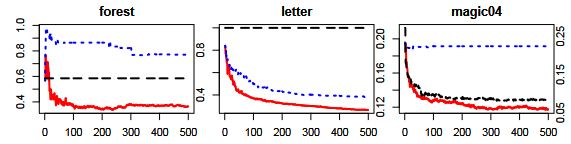
\includegraphics[width=0.8\linewidth]{images/MMperformance.JPG}
            \caption{\small Performance of \textcolor{red}{MM} in \cite{mukherjee2011theory}}
            \label{fig:Performance}
        \end{figure}
    \end{center}
    \begin{figure}

    \end{figure}
\end{frame}

\begin{frame}{Outlook}
    \textbf{\textcolor{red}{Restrictions:}}
    \begin{itemize}
        \item Loss function has to be convex.
        \item Sensitive to Outliers and Noise.
    \end{itemize}
    \bigbreak
    \textbf{\textcolor{blue}{Solutions and modern Methods:}}
    \begin{itemize}
        \item Boosting Algorithms that minimize non-convex error \cite{pfetsch2020ipboost} exist!
        \item A modern approach is Gradient-Boosting which essentially does Gradient-decent in function space $\mathcal{H}$
    \end{itemize}

\end{frame}

\begin{frame}{References}
    \printbibliography
\end{frame}

%%%%%%%%%%%%%%%%%% End of Presentation %%%%%%%%%%%%%%%%%


\end{document}